\chapter{Architecture and System Design}
\label{chap:architecture}

This chapter aims to explore the architecture and design of the CardioSync framework, building upon the problem statement from Chapter 1 and with the aid of literature review in Chapter 2.

\noindent The central issue addressed in this thesis revolves around the existing FreeBie architecture, which grants intermittent power capabilities solely to one end device of a BLE network. To extend this to both end devices, the challenge lies in devising a synchronisation mechanism within a battery-free architecture and crafting an efficient wake-up scheduling strategy.

\noindent In response to these challenges, this chapter outline the architectural evolution from FreeBie to CardioSync, highlighting the transformative integration of the framework. Also this chapter, we provide a thorough analysis of the proposed architecture, focusing on key components, interactions, and overall design concepts.

\noindent Furthermore, to aid in understanding the conceptual landscape, \autoref{fig:architecture} illustrates the high-level architecture of the CardioSync framework within the existing FreeBie model.


\section{Overview of Existing FreeBie Model}
Before delving into the details of the CardioSync framework, it is essential to establish a foundation by understanding the existing FreeBie model. FreeBie, a notable advancement in the field of battery-less embedded systems, provides the groundwork, incorporating innovative energy harvesting techniques and intermittent operation strategies to enable devices to function without conventional batteries.  

\noindent From Figure \ref{fig:architecture}, it can be noted that the whole model of FreeBie is built on top of any normal IoT embedded systems architecture with BLE networking stack. FreeBie includes components like FRAM, External RTC, Time-Deterministic Checkpointing and Restore, and Power Control, all of which leverage the base system's real-time virtualization of time and peripherals to enable unobstructed communication on an intermittently-powered budget \cite{de2022Intermittently}.

\begin{figure}[H]
    \centering
    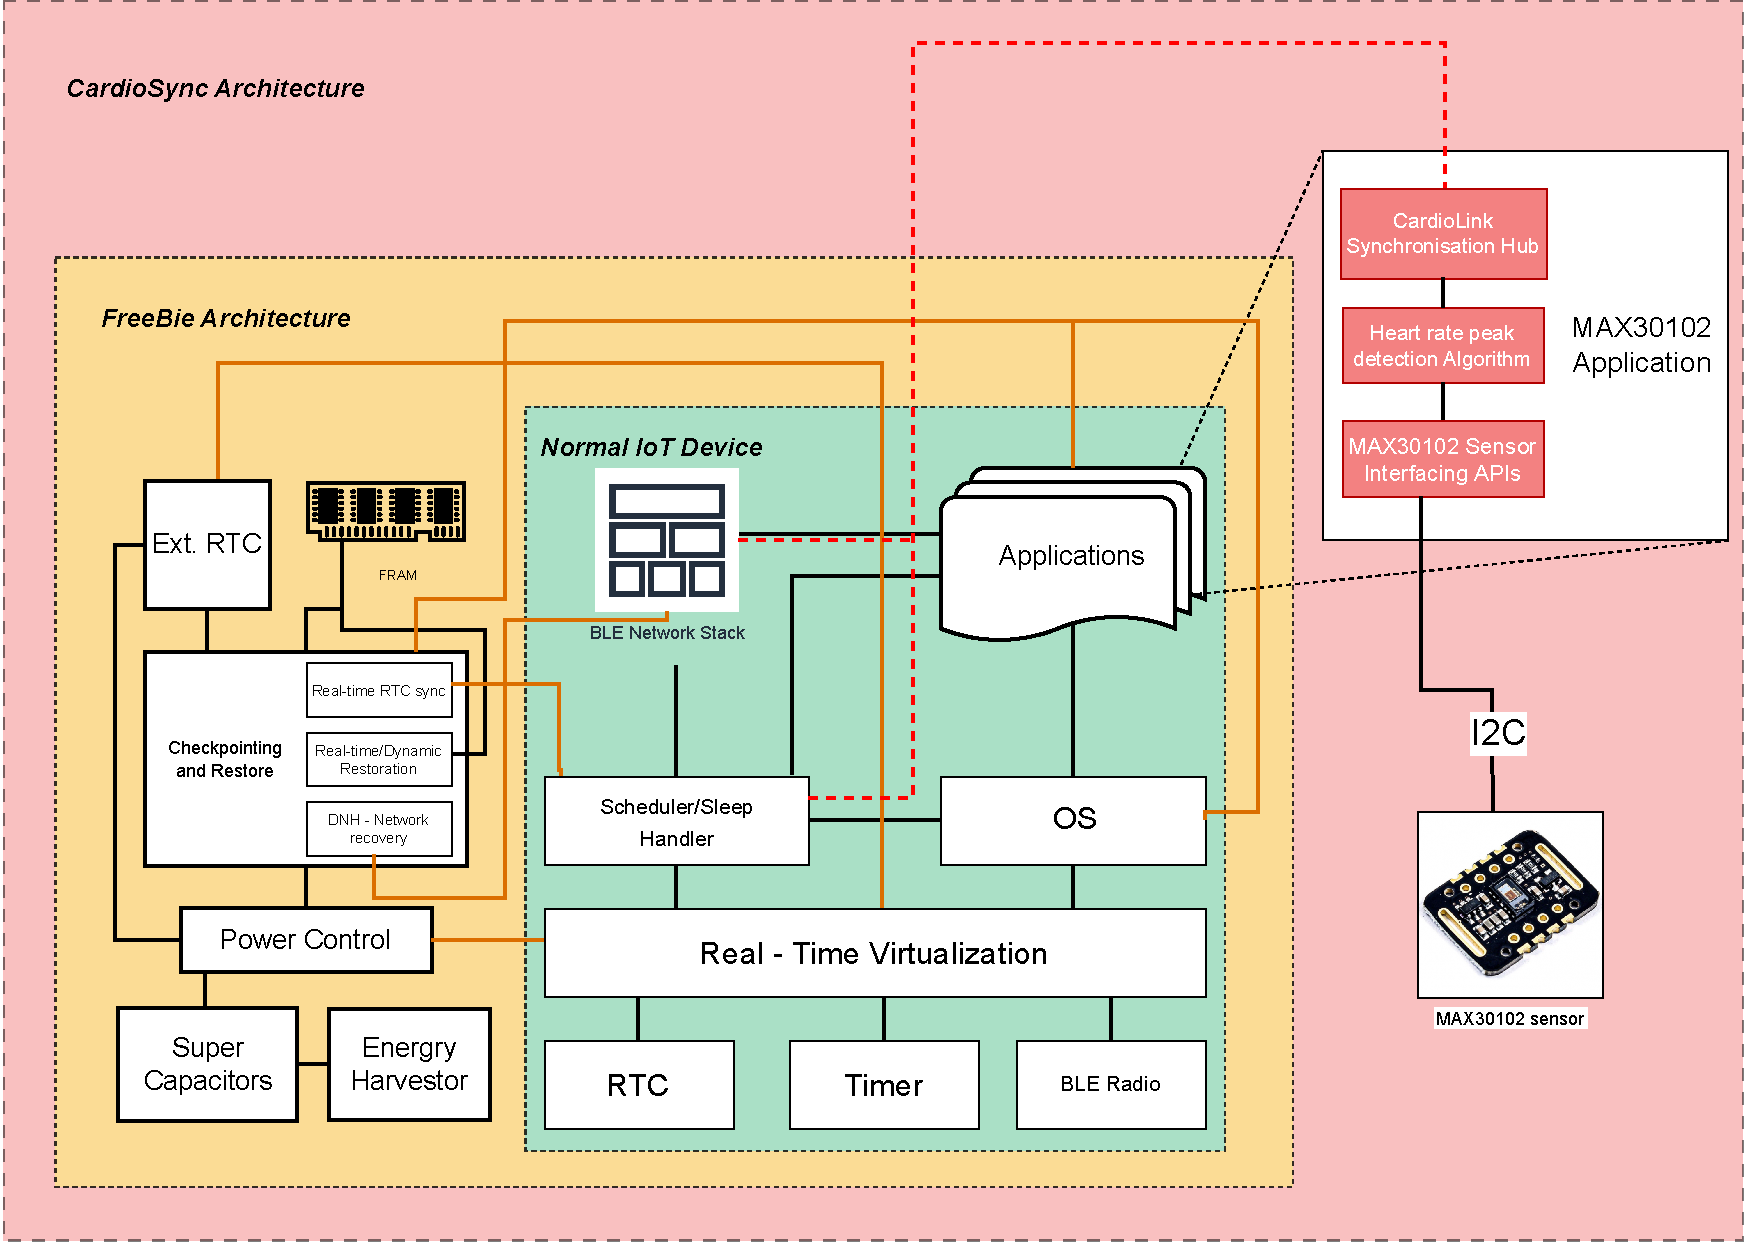
\includegraphics[width=\linewidth]{chapters/Architecture/architecture.pdf}
    \caption{High Level Architecture of the CardioSync framework}
    \label{fig:architecture}
\end{figure}

\noindent Each of these components serve a critical role on achieving the battery less operation:
\begin{itemize}
    \item \textbf{FRAM (Ferroelectric RAM):} FRAM is a non-volatile memory technology that offers high read/write speeds and low power consumption. It stores data and program code, ensuring persistence during power cycles. FRAM preserves memory sections during each checkpoint and stores context across separate allocated regions for OS processes, Network processes, and Application processes.
    
    \item \textbf{External RTC (Real-Time Clock):} The external RTC provides accurate timekeeping even during device power-off periods. This time reference is vital for synchronisation and event scheduling. The external RTC remains always powered through onboard capacitors and can control processor power domains using the Power switch and Power control module.
    
    \item \textbf{Time-Deterministic Checkpointing and Restore:} This component maintains data integrity by regularly capturing the device's state. In cases of power disruptions, the system can restore to a known state, preventing data loss and ensuring system consistency. It leverages External RTC and FRAM for uninterrupted atomic operations.
    
    \begin{itemize}
        \item \textit{Real-time RTC sync:} This subcomponent synchronises the Ext. RTC with the onboard RTC during each real-time operation resumption from power-off state. It uses FRAM to store the synchronising time \(T_{Sync}\) in the OS context.
        \item \textit{Real-time/Dynamic Restoration:} Upon resuming from power-off state, this component restores processes from FRAM for OS processes, network processes, and real-time application processes, as scheduled by the scheduler.
        \item \textit{Dynamic Handling of Network Connection:} Responsible for network recovery and dynamic network adaptation, this subcomponent ensures network recovery in unexpected power-offs and adapts to energy conditions while maintaining connection.
    \end{itemize}
    
    \item \textbf{Power Control:} Governing power state transitions, power control mechanisms by managing power-on timings, task execution, and low-power modes.
    
    \item \textbf{Super Capacitors and Energy Harvesters:} Integral to FreeBie's energy autonomy, super capacitors and energy harvesters contribute to storing and harnessing energy from ambient sources.
\end{itemize}

\noindent Leveraging these components, FreeBie achieves its ultimate objective of enabling seamless BLE communication and operation within an intermittently-powered paradigm \cite{de2022Intermittently}.

\section{Identification of Areas for Improvement}
While FreeBie represents a significant advancement in the realm of battery-less embedded systems, the intermittent power operation of devices within a communication network introduces specific challenges. These challenges are particularly pronounced when both end devices within the network operate on intermittent power sources. In response, significant areas for improvement have been identified, prompting the development of the CardioSync framework.

\noindent The key areas for improvement within the FreeBie model include:

\begin{itemize}
    \item \textbf{Bidirectional Intermittent Operation:} The original FreeBie architecture features asymmetric operation with periodic advertisement, where one end device intermittently operates while the other remains continuously powered. CardioSync should aim to extend energy efficiency to both end devices, enabling bidirectional intermittent operation.
    
    \item \textbf{Dynamic Wake-Up Scheduling:} Intermittent operation necessitates strategic wake-up scheduling to optimize BLE connection setup and minimize energy consumption. The complexity increases when both end devices experience intermittent power cycles. The architecture in design should aim to create an intelligent wake-up strategy that aligns with the dynamic power availability of intermittently-powered devices, ensuring synchronised connection setup.

\end{itemize}

\noindent By distinguishing these areas for improvement, the CardioSync framework aims to enable robust synchronisation between intermittently-powered devices, using external fixed common clock pulse. The figure \ref{fig:freebie_vs_cardiosync} highlights the difficulty encountered in establishing a connection between intermittent end devices using the FreeBie architecture. Additionally, it showcases the approach used by CardioSync to address this obstacle via the utilization of external pulse.

\begin{figure}[H]
    \centering
    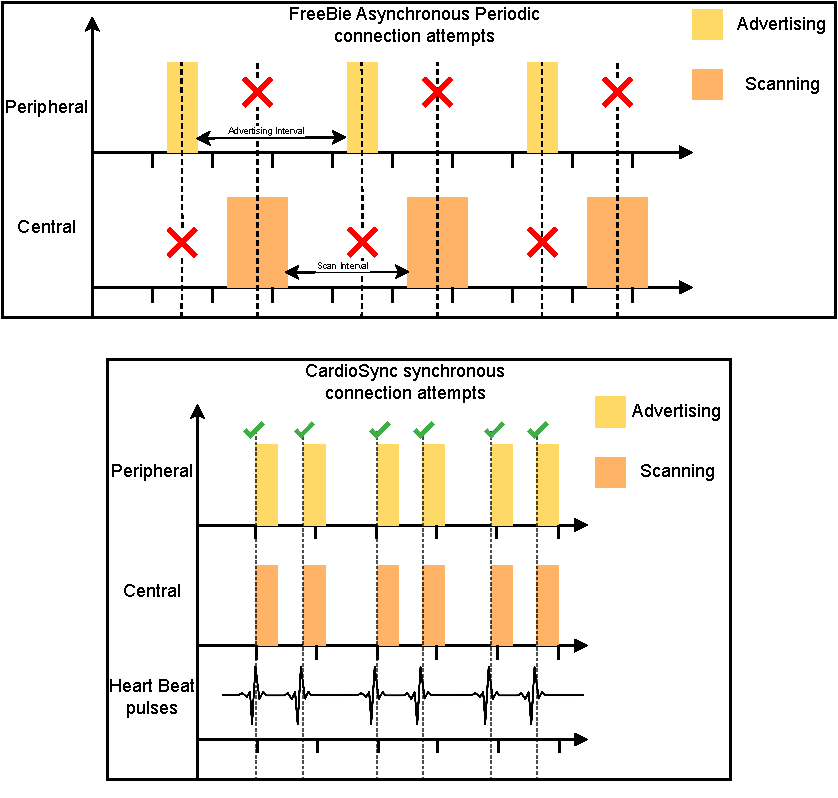
\includegraphics[width=0.6\linewidth]{chapters/Architecture/Freebie Vs. CardioSync.pdf}
    \caption{Conceptual diagram showing connection setup events of both end devices in FreeBie vs. CardioSync framework}
    \label{fig:freebie_vs_cardiosync}
\end{figure}

\section{Proposed Contribution - CardioSync Framework Integration}
The CardioSync framework represents a novel approach to address the synchronisation and connectivity challenges inherent in battery-less embedded systems. By integrating heart rate peak detection algorithm with Bluetooth Low Energy (BLE), CardioSync establishes synchronisation points and enhances connectivity even in the absence of continuous power.

\noindent The integration of the CardioSync framework is structured around the following key aspects:

\begin{itemize}
    \item \textbf{Heart Rate Peak Detection Algorithm:} CardioSync leverages advanced heart rate peak detection algorithms. These algorithms interpret heart rate data collected from the MAX30102 sensor interfaced with the MCU. The detection of heart rate peaks serves as the basis for scheduling synchronisation events, allowing intermittently-powered devices to synchronise their activities.
    
    \item \textbf{Synchronised BLE Connection:} In tandem with heart rate pulse detection, CardioSync synchronises BLE connection functionalities and enables the orchestrated scheduling of BLE advertising and scanning events that aligns with heart rate patterns, enhancing both connectivity and energy efficiency.
    
    \item \textbf{Establishing synchronisation Points:} The CardioSync framework introduces the concept of synchronisation points, which are strategically defined moments in time based on heart rate peaks. These points become the triggers for connection setup instances.
        
\end{itemize}

\noindent After a comprehensive review of available low-power heart rate detection sensors, the MAX30102 sensor from Maxim Integrated was selected as the heart rate monitor for the CardioSync framework. The MAX30102 sensor, consuming less than 1 mW and featuring low shutdown current around 0.7 \(\mu\)A, fits seamlessly with CardioSync's design goals.

\section{Architectural Changes and Components}
The CardioSync framework extends the FreeBie architecture to introduce a real-time application named MAX30102 application. This addition brings forth new components that contribute to the key aspects discussed:

\begin{itemize}
    \item \textbf{MAX30102 Sensor Interfacing APIs:} These APIs facilitate interaction between the MAX30102 sensor and the MCU using nRF5 SDK's TWI module to communicate through \(I^2C\) interface. They enable the collection of sensor data, forming the foundation for the heart rate peak detection algorithm.
    
    \item \textbf{Heart Rate Peak Detection Algorithm:} This algorithm processes the sensor data from the MAX30102 sensor and accurately detects heart rate peaks. The algorithm's outputs are pivotal in establishing synchronisation points and facilitating precise BLE adversting or scanning initiation instances.
    
    \item \textbf{CardioLink synchronisation Hub:} Serving as the central hub, this component handles the heart rate peaks processing, synchronisation points and BLE connection initiations. It ensures coordination between heart rate peak detection algorithm and scheduling of BLE advertising or scanning through existing FreeBie architecture's scheduler. This ensures synchronisation with sleep and wake-up intervals aligned with heart rate intervals instead of periodic advertisement or scan. This key component enables both end devices to be intermittent and still able to establish a BLE connection.
    
\end{itemize}

\section{High-Level Operation Flow}
The CardioSync framework operates through a systematic sequence of steps, integrating the heart rate peak detection algorithm with BLE stack as follows:

\begin{enumerate}
    \item \textbf{Sensor Data Acquisition:} The process begins with the acquisition of sensor data through dedicated APIs. The MAX30102 sensor reads the IR sensor values, capturing blood flow information. These values are temporarily stored in a buffer.
    
    \item \textbf{Heart Rate Peak Detection:} The sensor data is then fed into the heart rate peak detection algorithm. This algorithm discerns peaks indicative of heart rate activity from the provided data.
    
    \item \textbf{CardioLink Hub Verification:} Once a heart rate peak is detected, the CardioLink synchronisation Hub steps in. It verifies whether the peak corresponds to a new occurrence. This verification is based on the PalRTCTicks linked with each peak.
    
    \item \textbf{Instant Advertisement/Scanning Scheduling:} When a verified heart rate peak is detected, the CardioLink Hub orchestrates instantaneous scheduling of BLE advertising or scanning events. This scheduling leverages the FreeBie architecture, enabling connection instances aligned with heart rate intervals.
    
    \item \textbf{Heart Rate Interval Calculation:} The CardioSync framework calculates the heart rate interval based on the timing of multiple detected heart rate peaks. This interval defines the temporal spacing between synchronisation points.
    
    \item \textbf{Sensor Data Collection Pause:} Upon calculating the heart rate interval using multiple peaks, the sensor data collection process is temporarily paused. This pause ensures accurate synchronisation and prevents unnecessary data acquisition.
    
    \item \textbf{synchronisation Point Establishment:} Using the calculated heart rate interval, synchronisation points are established. These synchronisation points serve as triggers for possible connection establishment instances between intermittently-powered devices.
    
    \item \textbf{Scheduled Advertisement/Scanning:} With synchronisation points in place, the CardioLink Hub schedules BLE advertising or scanning events within the heart rate interval. This ensures connectivity aligned with the heart rate patterns.
    
    \item \textbf{Iteration and Adaptation:} The process continues to iterate, adapting to the dynamic heart rate patterns and power availability till the connection setup is complete. The framework ensures synchronisation, connectivity even in intermittent power scenarios.
\end{enumerate}

\noindent The workings of the algorithm and the CardioSync framework will be elaborated upon in the upcoming Implementation chapter, providing a comprehensive understanding of the operational intricacies.
